\section{Digital Interfaces}\label{sec:digital-interfaces}

	All sensoring data was obtained using analog channels, some digital channels will be reserved on the board in order to provide another type of sensing and control.

	\subsection{Digital Outputs}\label{ssec:digital-outputs}

		\subsubsection{Low-side Driver}\label{sssec:digital-outputs-low-side-driver}

			Item \ref{itm:func-req-11} from Section \ref{sec:functionalRequirements} states that the system must have a digital output channel to control a relay). According to \cite{songle-relay-datasheet}, a standard 5V relay will have a nominal current of 89.3mA, the microcontroller's datasheet \cite{atmega32u4-datasheet} says that the maximum DC current per I/O pin is 40mA though. Hence it is not possible to activate a relay connected directly to a MCU's I/O pin.
			\par 
			In order to solve this a relay driver circuit needs to be used, in this case a low side mosfet driver similar to the one from Figure \cite{pmos-low-side-driver} will be used.

			\begin{figure}[htbp]
				\centering
				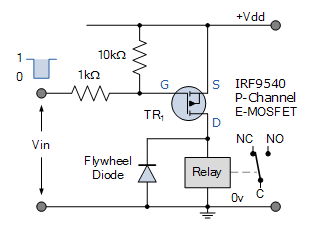
\includegraphics[width=.8\textwidth]{figuras/fig-pmos-low-side-driver.png}
				\caption{PMOS low side driver \cite{pmos-low-side-driver}}
				\label{fig:pmos-low-side-driver}
			\end{figure}

			This is a low-side driver, when the PMOS is submitted to a high logic level (5V) in it's gate it will enter on the cutoff region and will not conduct current, hence not activating the relay. On the other hand, when a low logic level (0V) is applied to the device's gate it will enter the saturation region and will conduct current, hence activating the relay.

		\subsubsection{Digital Output Circuit}\label{sssec:digital-output-circuit}

			The digital output circuit will be very similar to the one from Figure \ref{fig:pmos-low-side-driver}. The power supply connected to the mosfet will be the 5V source (check Section \ref{sssec:5v-supply}), on the PMOS drain there will be a TVS diode (SMBJ12A from \textit{Littlefuse} \cite{smbj12a-datasheet}) (check Section \ref{sssec:tvsTransientProtection}), this TVS will protect the PMOS from reverse current and from overvoltages. Figure \ref{fig:digital-output-circuit} show the equivalent circuit for the digital output.

			\begin{figure}[htbp]
				\centering
				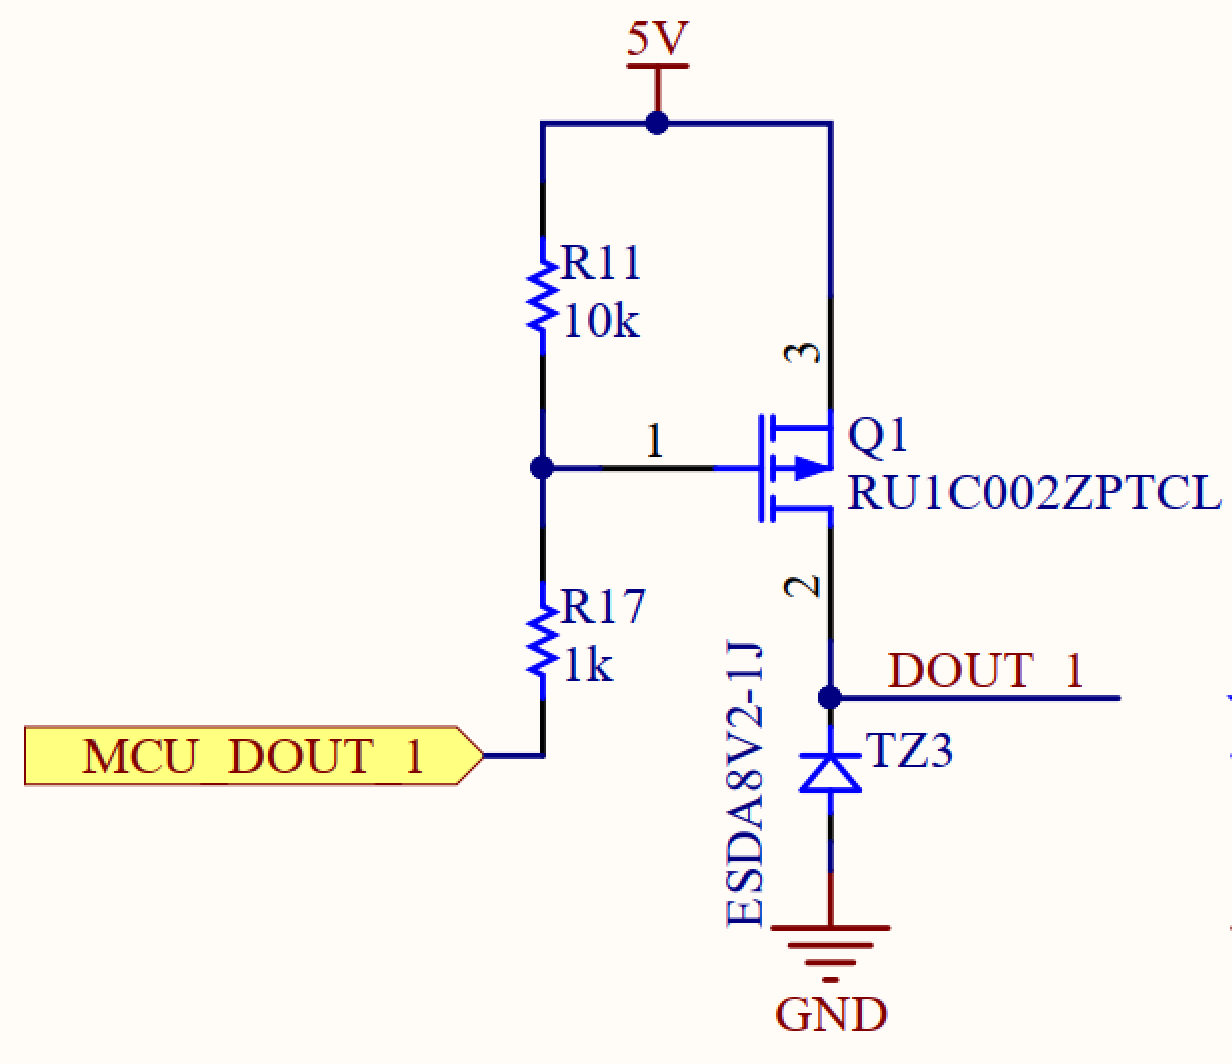
\includegraphics[width=.8\textwidth]{figuras/fig-digital-output-circuit.png}
				\caption{Digital Output Circuit}
				\label{fig:digital-output-circuit}
			\end{figure}

			The selected PMOS is the NDS332P from \textit{Fairchild} \cite{nds332p-datasheet}, it has a maximum operating continuos current of 1A, maximum gate threshold voltage of 1V, maximum drain-source voltage of 20V and maximum gate source voltage of $\pm$8V. It is adequate for this purpose. Resistor R7 is used to limit the magnitude of the current spike that can occur when a driver switches fast and has to charge or discharge a large gate capacitance. Resistor R5 is a pull-up for the gate, it will ensure that the PMOS will be in cutoff region if there is no input for the MCU. Resistor R8 is optional, for activating relays it is not needed, but other loads may require a pull-down, that is why it was placed on the PMOS drain. It was decided to keep any relay out of the board to save space. Moreover, keeping the relay out of the board gives room for using this digital output for other purposes. Although the project Requirements only specifies two digital ouputs, as there were unused MCU digital ports, a third digital output will also be placed on the PCB layout. 

	\subsection{Digital Inputs}\label{ssec:digital-inputs}

		This project does not have any requirement for digital inputs. However, in order to make the project more versatile for the future, making it able to capture switch states and possible external event, three digital inputs were added to the PCB. Figure \ref{fig:digital-input-circuit} show the circuit to interface the digital inputs.

			\begin{figure}[htbp]
				\centering
				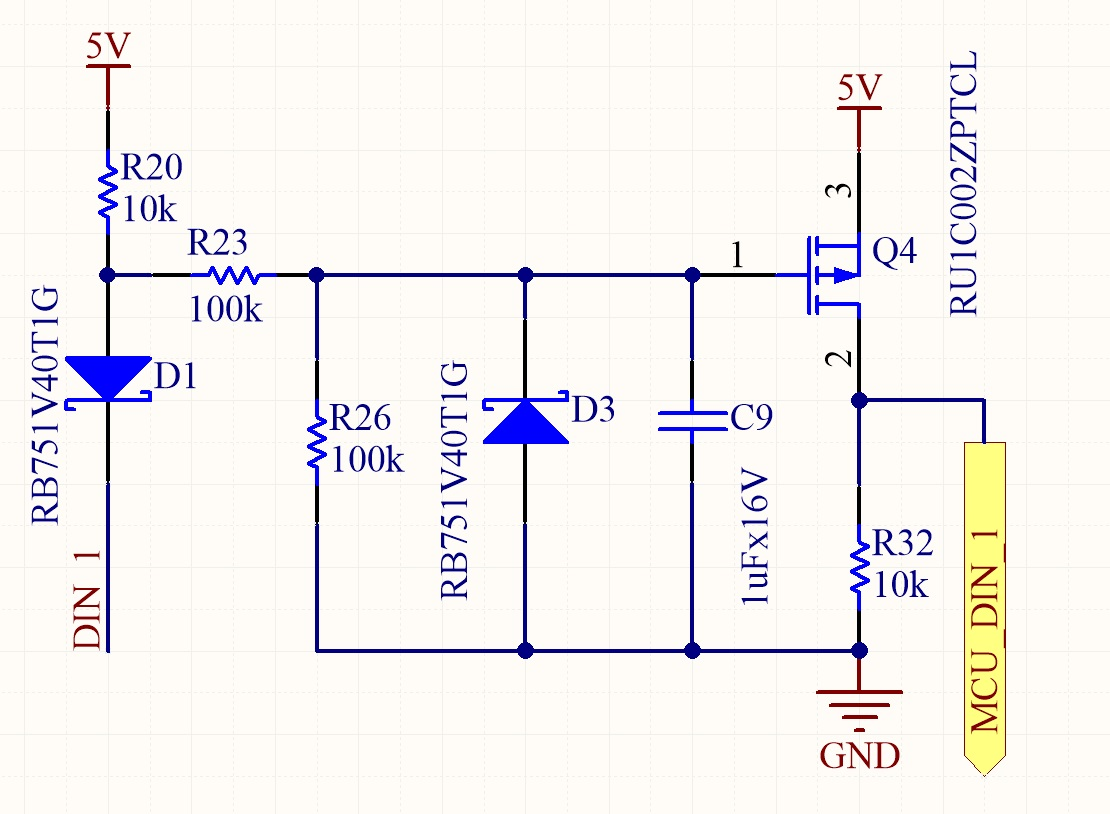
\includegraphics[width=.8\textwidth]{figuras/fig-digital-input-circuit}
				\caption{Digital Input Circuit}
				\label{fig:digital-input-circuit}
			\end{figure}

		According to \cite{RB751V40T1-datasheet}, the schottky diode on the input has a reverse voltage of 30V and a foward voltage of 280mV. When a voltage lower than 280mV is present on the input, the voltage on the PMOS gate will be lower than than its threshold (according to device's datasheet \cite{RU1C002ZP-datasheet}) the PMOS will start to conduct current and the signal \textit{MCU$\_$DIN$\_$1} will go to 5V. When the voltege on the input is higher than 280mV, the voltage on the PMOS gate will be higher than the treshold voltage and the PMOS will not conduct current, therefore, because of the pull down resistor R32, the signal \textit{MCU$\_$DIN$\_$1} will go to 0V.